\documentclass[11pt]{article}


\usepackage[margin=1in]{geometry}
\usepackage{amsthm,amsmath,amsfonts,amssymb}
\usepackage[authoryear]{natbib}
\usepackage{xcolor}
\usepackage{float}
\usepackage{booktabs}
\usepackage{tikz}
\usetikzlibrary{bayesnet}
\usetikzlibrary{positioning}
\usepackage[citecolor=blue,urlcolor=blue]{hyperref}
\usepackage{graphicx}


\usepackage{etoolbox}
\usepackage{bbm}


\RequirePackage{amsthm,amsmath,amsfonts,amssymb}
\RequirePackage[authoryear]{natbib}
\usepackage{float}
\usepackage{booktabs}
\usepackage{multirow}
\usepackage{longtable}
\usepackage{graphicx}

\usepackage{hyperref}
\hypersetup{
    colorlinks,
    citecolor=black,
    filecolor=black,
    linkcolor=black,
    urlcolor=black
}


\renewcommand{\thesection}{S\arabic{section}}
\renewcommand{\thesubsection}{S\arabic{section}.\arabic{subsection}}
\renewcommand{\thesubsubsection}{S\arabic{section}.\arabic{subsection}.\arabic{subsubsection}}
\makeatletter
\renewcommand{\thefigure}{S\@arabic\c@figure}
\renewcommand{\thetable}{S\@arabic\c@table}
\makeatother
\makeatletter
\renewcommand{\theequation}{S\@arabic\c@equation}
\makeatother


\def\DMO{\DeclareMathOperator}
\def\oper#1{\csdef{#1}{\operatorname{#1}}}
\forcsvlist\oper{GL,SL,deg,Hom,End,Vect,Mod,Rep,Ker,Im,Id}
\def\prob{\operatorname{P}}
\def\Gam{\operatorname{Gamma}}
\def\Mult{\operatorname{Multinomial}}
\def\Dir{\operatorname{Dirichlet}}
\def\Bern{\operatorname{Bernoulli}}
\def\pg{\operatorname{PG}}
\def\Ex{\operatorname{E}}
\def\VI{\operatorname{VI}}
\def\Var{\operatorname{Var}}
\def\diag{\operatorname{diag}}
\def\vect{\operatorname{vec}}
\def\cl{\operatorname{cl}}
\def\nsub{\operatorname{n}}

% Mathbb Letters. Usage: \bA
\def\defbb#1{\csdef{b#1}{\mathbb{#1}}}
\forcsvlist\defbb{A,B,C,D,E,F,G,H,I,J,K,L,M,N,O,P,Q,R,S,T,U,V,W,X,Y,Z}
\def\bk{\mathbbm k}

% Mathcal Letters. Usage: \cA
\def\defcal#1{\csdef{c#1}{\mathcal{#1}}}
\forcsvlist\defcal{A,B,C,D,E,F,G,H,I,J,K,L,M,N,O,P,Q,R,S,T,U,V,W,X,Y,Z}

% Greek letters
\def\al{\alpha}
\def\be{\beta}
\def\ga{\gamma}
\def\de{\delta}
\def\la{\lambda}
\def\ta{\tau}
\def\eps{\varepsilon}
\def\te{\theta}
\def\si{\sigma}
\def\om{\omega}
\def\Ga{\Gamma}
\def\De{\Delta}
\def\La{\Lambda}

% Bold Roman letters - lowercase
\def\bolda{\mathbf{a}}
\def\boldb{\mathbf{b}}
\def\boldc{\mathbf{c}}
\def\boldd{\mathbf{d}}
\def\bolde{\mathbf{e}}
\def\boldf{\mathbf{f}}
\def\boldg{\mathbf{g}}
\def\boldh{\mathbf{h}}
\def\boldi{\mathbf{i}}
\def\boldj{\mathbf{j}}
\def\boldk{\mathbf{k}}
\def\boldl{\mathbf{l}}
\def\boldm{\mathbf{m}}
\def\boldn{\mathbf{n}}
\def\boldo{\mathbf{o}}
\def\boldp{\mathbf{p}}
\def\boldq{\mathbf{q}}
\def\boldr{\mathbf{r}}
\def\bolds{\mathbf{s}}
\def\boldt{\mathbf{t}}
\def\boldu{\mathbf{u}}
\def\boldv{\mathbf{v}}
\def\boldw{\mathbf{w}}
\def\boldx{\mathbf{x}}
\def\boldy{\mathbf{y}}
\def\boldz{\mathbf{z}}

% Bold Roman letters - uppercase
\def\boldA{\mathbf{A}}
\def\boldB{\mathbf{B}}
\def\boldC{\mathbf{C}}
\def\boldD{\mathbf{D}}
\def\boldE{\mathbf{E}}
\def\boldF{\mathbf{F}}
\def\boldG{\mathbf{G}}
\def\boldH{\mathbf{H}}
\def\boldI{\mathbf{I}}
\def\boldJ{\mathbf{J}}
\def\boldK{\mathbf{K}}
\def\boldL{\mathbf{L}}
\def\boldM{\mathbf{M}}
\def\boldN{\mathbf{N}}
\def\boldO{\mathbf{O}}
\def\boldP{\mathbf{P}}
\def\boldQ{\mathbf{Q}}
\def\boldR{\mathbf{R}}
\def\boldS{\mathbf{S}}
\def\boldT{\mathbf{T}}
\def\boldU{\mathbf{U}}
\def\boldV{\mathbf{V}}
\def\boldW{\mathbf{W}}
\def\boldX{\mathbf{X}}
\def\boldY{\mathbf{Y}}
\def\boldZ{\mathbf{Z}}

% Bold Numbers 0-9
\def\bzero{\mathbf{0}}
\def\bone{\mathbf{1}}
\def\btwo{\mathbf{2}}
\def\bthree{\mathbf{3}}
\def\bfour{\mathbf{4}}
\def\bfive{\mathbf{5}}
\def\bsix{\mathbf{6}}
\def\bseven{\mathbf{7}}
\def\beight{\mathbf{8}}
\def\bnine{\mathbf{9}}

% Bold Greek letters - lowercase
\def\bsal{\boldsymbol{\alpha}}
\def\bsbet{\boldsymbol{\beta}}
\def\bsgam{\boldsymbol{\gamma}}
\def\bsdel{\boldsymbol{\delta}}
\def\bslam{\boldsymbol{\lambda}}
\def\bstau{\boldsymbol{\tau}}
\def\bseps{\boldsymbol{\epsilon}}
\def\bsthet{\boldsymbol{\theta}}
\def\bssig{\boldsymbol{\sigma}}
\def\bsom{\boldsymbol{\omega}}
\def\bsmu{\boldsymbol{\mu}}
\def\bskap{\boldsymbol{\kappa}}
\def\bsveps{\boldsymbol{\varepsilon}}
\def\bsphi{\boldsymbol{\phi}}
\def\bsvphi{\boldsymbol{\varphi}}
\def\bseta{\boldsymbol{\eta}}
\def\bspi{\boldsymbol{\pi}}
\def\bsnu{\boldsymbol{\nu}}
\def\bsrho{\boldsymbol{\rho}}

% Theorem environments (optional, adapt as needed)
\theoremstyle{plain}
\newtheorem{theorem}{Theorem}
\newtheorem{lemma}{Lemma}
\newtheorem{proposition}{Proposition}
\newtheorem{corollary}{Corollary}

\theoremstyle{definition}
\newtheorem{definition}{Definition}
\newtheorem{example}{Example}
\newtheorem{remark}{Remark}



\title{Bayesian Latent Class Regression and Variable Selection with
Applications to Sleep Patterns Data: Supplementary Material}
\author{}


\date{} 
\begin{document}


\maketitle
\tableofcontents

\section{Simulation Studies}
\subsection{Simulation 1: Parameter Estimates and Selection Results}

Table \ref{table:sim1_item_prob_estimates_full_LCR} contains the true and estimated values of the item probability parameters for the full LCR model for simulation 1, computed by posterior mean from Gibbs sampling. Table \ref{table:sim1_item_prob_estimates_itemsel} contains the estimates for the item probability parameters from the item selection model computed post-hoc. Table \ref{table:item_selection_results_sim_study1} contains posterior inclusion probabilities for each item variable in simulation 1. Figure \ref{fig:sim1_ridgeline_plot} contains a ridgeline plot illustrating the posterior distributions of the regression coefficients for the full LCR model without variable selection applied to simulation 1.

\begin{table}[H]
  \centering
\begin{tabular}{llcccc}
\toprule
\textbf{Var.} & \textbf{Cat.} & \textbf{True 1} & \textbf{Est. 1 (sd)} & \textbf{True 2} & \textbf{Est. 2 (sd)}  \\
\midrule
1 & 1 & 0.15 & 0.08 (0.03) & 0.70 & 0.74 (0.03)    \\
  & 2 & 0.25 & 0.30 (0.03) & 0.20 & 0.16 (0.02)   \\
  & 3 & 0.60 & 0.61 (0.04) & 0.10 & 0.10 (0.02)   \\
2 & 1 & 0.20 & 0.23 (0.03) & 0.55 & 0.55 (0.03)   \\
  & 2 & 0.35 & 0.32 (0.03) & 0.30 & 0.29 (0.03)   \\
  & 3 & 0.45 & 0.45 (0.04) & 0.15 & 0.15 (0.02)   \\
3 & 1 & 0.10 & 0.14 (0.03) & 0.80 & 0.82 (0.03)    \\
  & 2 & 0.15 & 0.15 (0.03) & 0.15 & 0.13 (0.02)    \\
  & 3 & 0.75 & 0.71 (0.04) & 0.05 & 0.05 (0.02)    \\
4 & 1 & 0.25 & 0.26 (0.03) & 0.45 & 0.44 (0.03)    \\
  & 2 & 0.40 & 0.35 (0.04) & 0.35 & 0.37 (0.03)    \\
  & 3 & 0.35 & 0.40 (0.04) & 0.20 & 0.19 (0.02)    \\
5 & 1 & 0.40 & 0.39 (0.04) & 0.40 & 0.44 (0.03)   \\
  & 2 & 0.50 & 0.53 (0.04) & 0.50 & 0.45 (0.03)   \\
  & 3 & 0.10 & 0.08 (0.02) & 0.10 & 0.11 (0.02)   \\
6 & 1 & 0.70 & 0.75 (0.03) & 0.70 & 0.72 (0.03)    \\
  & 2 & 0.10 & 0.07 (0.02) & 0.10 & 0.09 (0.02)   \\
  & 3 & 0.20 & 0.18 (0.03) & 0.20 & 0.19 (0.02)   \\
7 & 1 & 0.10 & 0.08 (0.02) & 0.10 & 0.09 (0.02)   \\
  & 2 & 0.50 & 0.50 (0.04) & 0.50 & 0.52 (0.03)    \\
  & 3 & 0.40 & 0.42 (0.04) & 0.40 & 0.38 (0.03)    \\  
8 & 1 & 0.33 & 0.28 (0.03) & 0.33 & 0.32 (0.03)  \\
  & 2 & 0.33 & 0.34 (0.03) & 0.33 & 0.34 (0.03)    \\
  & 3 & 0.33 & 0.38 (0.04) & 0.33 & 0.34 (0.03)   \\  
\bottomrule
\end{tabular}
\caption{True and estimated values of the item probability parameters for the full LCR model for simulation 1.}
  \label{table:sim1_item_prob_estimates_full_LCR}
\end{table}

\begin{table}[H]
  \centering
\begin{tabular}{llcccc}
\toprule
\textbf{Var.} & \textbf{Cat.} & \textbf{True 1} & \textbf{Est. 1 (sd)} & \textbf{True 2} & \textbf{Est. 2 (sd)}  \\
\midrule
1 & 1 & 0.15 & 0.08 (0.03) & 0.70 &  0.73 (0.03)   \\
  & 2 & 0.25 & 0.30 (0.03) & 0.20 &  0.16 (0.02)  \\
  & 3 & 0.60 & 0.62 (0.04) & 0.10 &  0.11 (0.02)  \\
2 & 1 & 0.20 & 0.23 (0.03) & 0.55 &  0.55 (0.03)   \\
  & 2 & 0.35 & 0.32 (0.03) & 0.30 &  0.29 (0.03)   \\
  & 3 & 0.45 & 0.45 (0.04) & 0.15 &  0.15 (0.02)  \\
3 & 1 & 0.10 & 0.13 (0.03) & 0.80 &  0.82 (0.03)  \\
  & 2 & 0.15 & 0.15 (0.03) & 0.15 &  0.13 (0.02)    \\
  & 3 & 0.75 & 0.72 (0.04) & 0.05 &  0.05 (0.02)  \\       
4 & 1 & 0.25 & 0.26 (0.03) & 0.45 &  0.44 (0.03)   \\
  & 2 & 0.40 & 0.35 (0.04) & 0.35 &  0.37 (0.03)   \\
  & 3 & 0.35 & 0.40 (0.04) & 0.20 &  0.19 (0.02)   \\
5 & 1 & 0.40 & 0.40 (0.04) & 0.40 &  0.44 (0.03) \\
  & 2 & 0.50 & 0.52 (0.04) & 0.50 &  0.46 (0.03)  \\
  & 3 & 0.10 & 0.08 (0.02) & 0.10 &  0.11 (0.02)  \\
6 & 1 & 0.70 & 0.74 (0.04) & 0.70 &  0.72 (0.03)   \\
  & 2 & 0.10 & 0.07 (0.02) & 0.10 &  0.09 (0.02)  \\
  & 3 & 0.20 & 0.18 (0.03) & 0.20 &  0.19 (0.02) \\
7 & 1 & 0.10 & 0.08 (0.02) & 0.10 &  0.09 (0.02)  \\
  & 2 & 0.50 & 0.50 (0.04) & 0.50 &  0.52 (0.03)   \\
  & 3 & 0.40 & 0.42 (0.04) & 0.40 &  0.39 (0.03)  \\  
8 & 1 & 0.33 & 0.29 (0.03) & 0.33 &  0.32 (0.03) \\
  & 2 & 0.33 & 0.34 (0.04) & 0.33 &  0.34 (0.03)  \\
  & 3 & 0.33 & 0.34 (0.04) & 0.33 &  0.34 (0.03)  \\  
\bottomrule
\end{tabular}
\caption{Estimated values of the item probability parameters for the item selection model for simulation 1.}
  \label{table:sim1_item_prob_estimates_itemsel}
\end{table}


\begin{table}[H]
\centering
\begin{tabular}{ccccccccc}
\hline
Variable & 1 & 2 & 3 & 4 & 5 & 6 & 7 & 8 \\
\hline
PIP (item) & 1.00 & 1.00 & 1.00 & 1.00 & 0.08 & 0.02 & 0.03 & 0.04  \\
PIP (simul) & 1.00 & 1.00 & 1.00 & 1.00 & 0.07 & 0.02 & 0.03 & 0.04  \\
\hline
\end{tabular}
\caption{Posterior inclusion probabilities (PIP) for each item variable in the LCR model for simulation 1. 
PIP (item): item selection alone; PIP (simul): simultaneous selection. }\label{table:item_selection_results_sim_study1}
\end{table}

\begin{figure}[H]
    \centering
    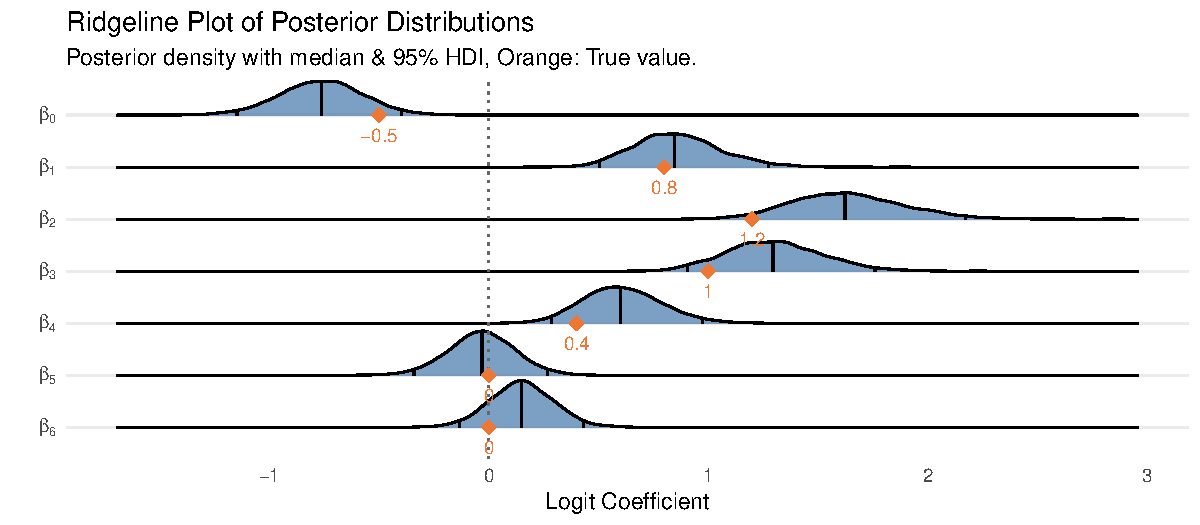
\includegraphics[width=\linewidth]{sim_study_plots/ridgeline_plot_sim1.pdf}
    \caption{Ridgeline plots of posterior distribution of regression coefficients for simulation 1.}
    \label{fig:sim1_ridgeline_plot}
\end{figure}



\subsection{Simulation 2: Parameter Estimates and Selection Results}
Table \ref{table:sim2_item_prob_estimates_itemsel} contains the true and estimated values of the item probability parameters for the collapsed LCR model for simulation 2, computed post-hoc. Table \ref{table:item_selection_results_sim_study2} contains posterior inclusion probabilities for each item variable in simulation 2. Figure \ref{fig:sim2_ridgeline_plot} contains a ridgeline plot illustrating the posterior distributions of the regression coefficients for the LCR model with item selection only applied to simulation 2.
\begin{table}[H]\centering
\begin{tabular}{llcccccc}
\toprule
\textbf{Var.} & \textbf{Cat.} & \textbf{True 1} & \textbf{Est. 1 (sd)} & \textbf{True 2} & \textbf{Est. 2 (sd)} & \textbf{True 3} & \textbf{Est. 3 (sd)} \\
\midrule
1 & 1 & 0.15 & 0.18 (0.03) & 0.60 & 0.58 (0.04) & 0.80 & 0.80 (0.05)   \\
  & 2 & 0.85 & 0.82 (0.03) & 0.40 & 0.42 (0.04) & 0.20 & 0.20 (0.05)   \\
2 & 1 & 0.25 & 0.24 (0.03) & 0.45 & 0.45 (0.04) & 0.70 & 0.77 (0.06)  \\
  & 2 & 0.75 & 0.76 (0.03) & 0.55 & 0.55 (0.04) & 0.30 & 0.23 (0.06)   \\
3 & 1 & 0.70 & 0.70 (0.04) & 0.20 & 0.23 (0.03) & 0.65 & 0.71 (0.08)   \\
  & 2 & 0.30 & 0.30 (0.04) & 0.80 & 0.77 (0.03) & 0.35 & 0.29 (0.08)   \\
4 & 1 & 0.10 & 0.08 (0.02) & 0.35 & 0.39 (0.04) & 0.70 & 0.64 (0.07)   \\
  & 2 & 0.25 & 0.28 (0.03) & 0.40 & 0.34 (0.04) & 0.20 & 0.26 (0.06)   \\
  & 3 & 0.65 & 0.64 (0.04) & 0.25 & 0.27 (0.03) & 0.10 & 0.09 (0.04)   \\
5 & 1 & 0.20 & 0.18 (0.03) & 0.25 & 0.29  (0.04) & 0.65 & 0.66 (0.07)  \\
  & 2 & 0.15 & 0.17 (0.03) & 0.60 & 0.59  (0.04) & 0.25 & 0.25 (0.06)  \\
  & 3 & 0.65 & 0.65 (0.04) & 0.15 & 0.12  (0.03) & 0.10 & 0.09 (0.04)  \\
6 & 1 & 0.15 & 0.11 (0.03) & 0.50 & 0.45  (0.03) & 0.75 & 0.79 (0.06)   \\
  & 2 & 0.20 & 0.21 (0.03) & 0.35 & 0.38  (0.04) & 0.15 & 0.13 (0.05)  \\
  & 3 & 0.65 & 0.68 (0.04) & 0.15 & 0.16  (0.03) & 0.10 & 0.09 (0.03)  \\
7 & 1 & 0.10 & 0.10 (0.02) & 0.25 & 0.25  (0.03) & 0.60 & 0.51 (0.06)  \\
  & 2 & 0.15 & 0.13 (0.03) & 0.35 & 0.33  (0.03) & 0.25 & 0.28 (0.06)   \\
  & 3 & 0.25 & 0.23 (0.03) & 0.25 & 0.25  (0.03) & 0.10 & 0.15 (0.04)   \\  
  & 4 & 0.50 & 0.53 (0.04) & 0.15 & 0.17  (0.03) & 0.05 & 0.06 (0.03)   \\
8 & 1 & 0.15 & 0.20 (0.03) & 0.20 & 0.20  (0.03) & 0.55 & 0.67 (0.07)  \\
  & 2 & 0.20 & 0.14 (0.03) & 0.45 & 0.45  (0.04) & 0.20 & 0.16 (0.06)   \\
  & 3 & 0.20 & 0.20 (0.03) & 0.25 & 0.26  (0.03) & 0.15 & 0.12 (0.04)  \\  
  & 4 & 0.45 & 0.46 (0.04) & 0.10 & 0.10  (0.02) & 0.10 & 0.05 (0.03)   \\
9 & 1 & 0.40 & 0.35 (0.04) & 0.40 & 0.43 (0.04) & 0.40 &  0.39 (0.07)   \\
  & 2 & 0.50 & 0.53 (0.04) & 0.50 & 0.46  (0.04) & 0.50 & 0.47 (0.07)   \\
  & 3 & 0.10 & 0.12 (0.02) & 0.10 & 0.11  (0.02) & 0.10 & 0.14 (0.04)   \\
10 & 1 & 0.70 & 0.72 (0.04) & 0.70 & 0.72  (0.04) & 0.70 & 0.68 (0.08)   \\
  & 2 & 0.10 & 0.10 (0.02) & 0.10 & 0.11 (0.02) & 0.10 & 0.15 (0.04)  \\
  & 3 & 0.20 & 0.18 (0.03) & 0.20 & 0.17 (0.03) & 0.20 & 0.17 (0.05)  \\
11 & 1 & 0.20 & 0.21 (0.03) & 0.20 & 0.20 (0.03) & 0.20 & 0.20 (0.05)  \\
  & 2 & 0.20 & 0.18 (0.03) & 0.20 & 0.20 (0.03) & 0.20 & 0.15 (0.04)  \\
  & 3 & 0.20 & 0.22 (0.03) & 0.20 & 0.20 (0.03) & 0.20 & 0.23 (0.05)  \\
  & 4 & 0.20 & 0.21 (0.03) & 0.20 & 0.20 (0.03) & 0.20 & 0.20 (0.05)   \\
  & 5 & 0.20 & 0.19 (0.03) & 0.20 & 0.20 (0.03) & 0.20 & 0.22 (0.05)  \\
12 & 1 & 0.10 & 0.15 (0.03) & 0.10 & 0.11 (0.02) & 0.10 & 0.08 (0.03) \\
  & 2 & 0.15 & 0.17 (0.03) & 0.15 & 0.13 (0.02) & 0.15 & 0.16 (0.04)  \\
  & 3 & 0.20 & 0.16 (0.03) & 0.20 & 0.20 (0.03) & 0.20 & 0.25 (0.05)  \\
  & 4 & 0.25 & 0.24 (0.03) & 0.25 & 0.21 (0.03) & 0.25  & 0.21 (0.05)  \\
  & 5 & 0.30 & 0.28 (0.03) & 0.30 & 0.34 (0.03) & 0.30 & 0.31 (0.06)  \\
13 & 1 & 0.20 & 0.20 (0.03) & 0.20 & 0.20 (0.03) & 0.20 & 0.23 (0.05)  \\
  & 2 & 0.30 & 0.27 (0.03) & 0.30 & 0.27 (0.03) & 0.30 & 0.33 (0.06)   \\
  & 3 & 0.30 & 0.31 (0.04) & 0.30 & 0.30 (0.03) & 0.30 & 0.29 (0.06)  \\
  & 4 & 0.10 & 0.10 (0.02) & 0.10 & 0.14 (0.03) & 0.10 & 0.09 (0.03)  \\
  & 5 & 0.10 & 0.11 (0.02) & 0.10 & 0.09 (0.02) & 0.10 & 0.06 (0.03)  \\
\bottomrule
\end{tabular}
\caption{True and estimated values of the item probability parameters for the item selection model for dataset 2.}
  \label{table:sim2_item_prob_estimates_itemsel}
\end{table}


\begin{table}[H]
\centering
\begin{tabular}{cccccccccccccc}
\hline
Variable & 1 & 2 & 3 & 4 & 5 & 6 & 7 & 8 & 9 & 10 & 11 & 12 & 13 \\
\hline
PIP (item) & 1.00 & 1.00 & 1.00 & 1.00 & 1.00 & 1.00 & 1.00 & 1.00 & 0.01 & 0.00 & 0.00 & 0.00 & 0.00 \\
PIP (simul) & 1.00 & 1.00 & 1.00 & 1.00 & 1.00 & 1.00 & 1.00 & 1.00 & 0.01 & 0.00 & 0.00 & 0.00 & 0.00 \\
\hline
\end{tabular}
\caption{Posterior inclusion probabilities (PIP) for each item variable in the LCR model for dataset 2. 
PIP (item): item selection alone; PIP (simul): simultaneous selection.}\label{table:item_selection_results_sim_study2}
\end{table}


\begin{figure}[H]
    \centering
    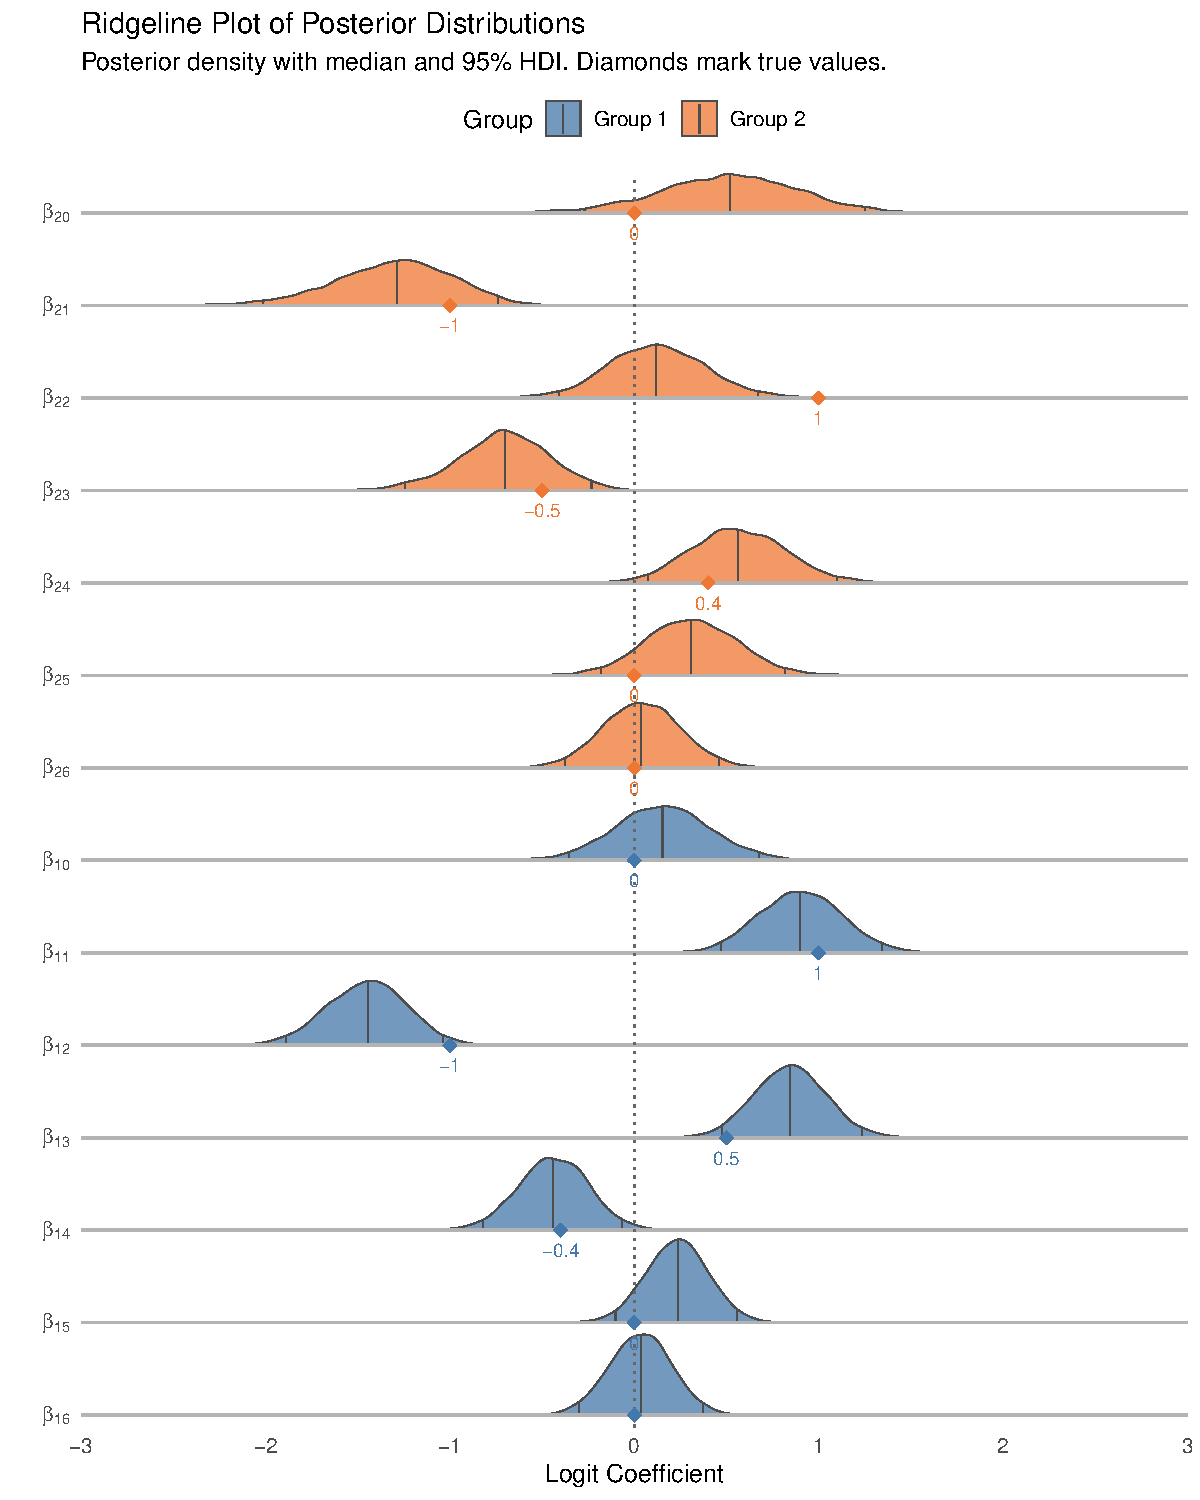
\includegraphics[width=\linewidth]{sim_study_plots/sim2_combined_ridgeline.pdf}
    \caption{Ridgeline plots of posterior distribution of regression coefficients for simulation 2.}
    \label{fig:sim2_ridgeline_plot}
\end{figure}


\section{CSHQ Sleep Data Analysis}
\subsection{Study Sample Characteristics}
Table \ref{table:demographic_diagnostic_table_CSHQ} contains demographic and diagnostic information for the sleep patterns dataset.
\begin{table}[H]
\centering
\begin{tabular}{llcc}
\toprule
 Demographic & &  $n$ & \% \\
\midrule
 Gender&  & \\
& Female &  69 & 46.6\\
& Male &   79 & 53.4\\
Diagnosis & & \\
& Neurotypical & 104 & 70.3 \\
& Neurodiverse & 44 & 29.7 \\
\bottomrule
Diagnosis/comorbidity (ND) & & $n$ & \% (ND group) \\
\midrule
ASD & & 19 & 43.18 \\
ID/ASD & & 6 & 13.64 \\
ADHD/ASD & & 5 & 11.36 \\
Dyslexia & & 3 & 6.82 \\
ADHD & & 2 & 4.55 \\
ASD/ADHD/Dyslexia & & 1 & 2.27 \\
ID/ASD/ADHD & & 1 & 2.27 \\
ASD/GDD & & 1 & 2.27 \\
ADHD/Dyslexia & & 1 & 2.27 \\
ID/Dyslexia & & 1 & 2.27 \\
ID & & 1 & 2.27 \\
Dyspraxia & & 1 & 2.27 \\
Tourette's & & 1 & 2.27 \\
Brain Abnormality & & 1 & 2.27 \\
\bottomrule
\end{tabular}
\caption{Demographic and diagnostic summary information for the CSHQ dataset (ND = neurodiverse, ASD = Autism Spectrum Disorder, ID = Intellectual Disability, GDD = Global Developmental Delay)}\label{table:demographic_diagnostic_table_CSHQ}
\end{table}
\subsection{Model Parameter Estimates}
Table \ref{table:CSHQ_item_prob_estimates_itemsel} contains estimates for the item probability parameters computed post-hoc for the sleep data LCR model with item selection. Table \ref{table:CSHQ_beta_estimates} contains posterior mean values for LCR regression coefficient parameters, along with sd and 95\% HDI values. Table \ref{table:CSHQ_beta_estimates_varsel} contains the estimates for the regression coefficient parameters for the ASD diagnosis variable with predictor selection.
\begin{longtable}{clccccc}
\caption{Estimated values of the item probability parameters for the item selection model for the CSHQ sleep data}
\label{table:CSHQ_item_prob_estimates_itemsel}\\
\toprule
\textbf{Variable} & & \textbf{Category}  & \textbf{Est. 1 (sd)}  & \textbf{Est. 2 (sd)}  & \textbf{Est. 3 (sd)} & \textbf{Est. 4 (sd)}  \\
\midrule
\endfirsthead

\multicolumn{7}{c}{\tablename\ \thetable\ -- \textit{Continued from previous page}} \\
\toprule
\textbf{Variable} & & \textbf{Category}  & \textbf{Est. 1 (sd)}  & \textbf{Est. 2 (sd)}  & \textbf{Est. 3 (sd)} & \textbf{Est. 4 (sd)}  \\
\midrule
\endhead

\midrule
\multicolumn{7}{r}{\textit{Continued on next page}} \\
\endfoot

\bottomrule
\endlastfoot
Bedtime Resistance &1 & 1  & 0.78 (0.06) & 0.77  (0.09) & 0.63 (0.10) & 0.68 (0.11)  \\
 & & 2  & 0.18 (0.05) & 0.18  (0.07) &  0.30 (0.09) & 0.27 (0.09)  \\
 & & 3  & 0.04 (0.03) &  0.05 (0.04) &  0.07 (0.05) & 0.04 (0.04) \\
&2 & 1  & 0.94 (0.03) &  0.75 (0.07) &  0.90 (0.05) & 0.51 (0.11)\\
 & & 2  & 0.02 (0.02) &  0.09 (0.05) &  0.07 (0.04) & 0.33 (0.10)\\
 & & 3  & 0.05 (0.03) &  0.16 (0.06) &  0.03 (0.03) & 0.16 (0.07)\\
&3 & 1  & 0.94 (0.03) &  0.75 (0.07) &  0.87 (0.06) & 0.43 (0.11)\\
&  & 2  & 0.02 (0.02) &  0.07 (0.04) &  0.09 (0.05) & 0.38 (0.10)\\
&  & 3  & 0.05 (0.03) &  0.18 (0.07) &  0.03 (0.03) & 0.19 (0.08)\\
 &5 & 1  & 0.89 (0.04) &  0.14 (0.07) &  0.77 (0.08) & 0.06 (0.04)\\
 & & 2  & 0.09 (0.04) &  0.38 (0.09) &  0.20 (0.08) & 0.25 (0.09)\\
&  & 3  & 0.02 (0.02) &  0.47 (0.08) &  0.04 (0.04) & 0.69 (0.10)\\

Sleep Onset Delay & & 1 & 0.58 (0.06) &  0.48  (0.09) & 0.15  (0.07) & 0.20 (0.09)\\
 & & 2 & 0.27 (0.06) &  0.41  (0.09) & 0.57  (0.09) & 0.35 (0.10)\\
 & & 3 & 0.15 (0.05) &  0.11  (0.05) &  0.28 (0.08) & 0.44 (0.10)\\
 
Sleep Duration  & 1 & 1  & 0.85 (0.05) &  0.65  (0.09) &  0.14 (0.07) & 0.08 (0.06)\\
 & & 2  & 0.12 (0.05) &  0.29  (0.09) &  0.55 (0.09) & 0.57 (0.11)\\
 & & 3  & 0.03 (0.02) &  0.06  (0.04) &  0.32 (0.09) & 0.35 (0.10)\\
  & 2 & 1  & 0.86 (0.05) &  0.65  (0.09) &  0.15 (0.07) & 0.05 (0.04)\\
 & & 2  & 0.10 (0.04) &  0.27  (0.09) & 0.53  (0.09) & 0.61 (0.10)\\
 & & 3  & 0.05 (0.03) &  0.09  (0.05) &  0.32 (0.09) & 0.35 (0.10)\\
   & 3 & 1  & 0.86 (0.05) &  0.74  (0.08) &  0.22 (0.08) & 0.29 (0.09)\\
 & & 2  & 0.11 (0.04) &  0.23  (0.08) &  0.54 (0.09) & 0.37 (0.10)\\
 & & 3  & 0.03 (0.02) &  0.03  (0.03) & 0.24  (0.08) & 0.33 (0.10)\\
 
 Sleep Anxiety  & 1 & 1  & 0.80 (0.05) &  0.14  (0.07) & 0.89  (0.06) & 0.09 (0.06) \\
 & & 2  & 0.13 (0.04) &  0.22  (0.07) &  0.06 (0.05) & 0.27 (0.05) \\
 & & 3  & 0.06 (0.03) &   0.63 (0.09) &  0.05 (0.04) & 0.64 (0.04) \\
  & 2 & 1  & 0.70 (0.06) &  0.35  (0.08) & 0.67  (0.09) & 0.31 (0.09) \\
 & & 2  & 0.20 (0.05) &  0.19  (0.07) &  0.12 (0.06) & 0.36 (0.10)\\
 & & 3  & 0.10 (0.04) &  0.46  (0.09) &  0.21 (0.08) & 0.32 (0.10)\\
   & 3 & 1  & 0.89 (0.04) &   0.11 (0.06) &  0.76 (0.08) & 0.06 (0.04)\\
 & & 2  & 0.08 (0.04) &  0.35  (0.08) &  0.20 (0.08) & 0.35 (0.10)\\
 & & 3  & 0.02 (0.02) &  0.54  (0.09) &  0.04 (0.04) & 0.59 (0.10)\\
    & 4 & 1  & 0.70 (0.06) &  0.63  (0.08) &  0.41  (0.09) & 0.14 (0.08) \\
 & & 2  & 0.27 (0.06) &  0.26  (0.07) & 0.40  (0.09) & 0.47 (0.10)  \\
 & & 3  & 0.03 (0.02) &  0.11  (0.05) & 0.19  (0.07) & 0.39 (0.10) \\
 
Night Waking  & 1 & 1  & 0.90 (0.04) &  0.48  (0.09) & 0.71  (0.09) & 0.18 (0.08)\\
 & & 2  & 0.08 (0.04) &  0.34  (0.08) &  0.20 (0.08) & 0.34 (0.10)\\
 & & 3  & 0.02 (0.02) &  0.17  (0.07) &  0.10 (0.07) & 0.48 (0.10)\\
  & 2 & 1  & 0.76 (0.06) &  0.33  (0.08) & 0.31  (0.08) & 0.10 (0.06)\\
 & & 2  & 0.21 (0.06) &  0.46  (0.09) &  0.33 (0.09) & 0.27 (0.09)\\
 & & 3  & 0.03 (0.02) &  0.21  (0.07) &  0.35 (0.09) & 0.63 (0.10)\\
   & 3 & 1  & 0.94 (0.03) &  0.64  (0.08) & 0.41  (0.10) & 0.36 (0.10)\\
 & & 2  & 0.04 (0.03) &  0.33  (0.08) &  0.25 (0.08) & 0.39 (0.10)\\
 & & 3  & 0.02 (0.02) &  0.03  (0.03) & 0.33  (0.09) & 0.25 (0.09)\\
 
 Parasomnias  & 1 & 1  & 0.91  (0.06) &  0.87  (0.09) &  0.81 (0.10) & 0.72 (0.11) \\
 & & 2  & 0.05 (0.03) &  0.08  (0.04) & 0.09  (0.05) & 0.12 (0.07)\\
 & & 3  & 0.05 (0.03) &  0.05 (0.04) &  0.09 (0.05) & 0.16 (0.07)\\
  & 2 & 1  & 0.68  (0.06) &  0.51  (0.09) & 0.77  (0.09) & 0.43 (0.10)\\
 & & 2  & 0.26 (0.06) &  0.46  (0.09) & 0.13  (0.07) & 0.49 (0.11)\\
 & & 3  & 0.05 (0.03) &  0.03  (0.03) & 0.10  (0.06) & 0.08 (0.06)\\
   & 3 & 1  & 0.48 (0.06) &  0.28  (0.08) & 0.27  (0.08) & 0.16 (0.08)\\
 & & 2  & 0.43 (0.06) &  0.54  (0.08) & 0.35  (0.09) & 0.34 (0.10)\\
 & & 3  & 0.10 (0.04) &  0.19  (0.07) & 0.38  (0.09) & 0.50 (0.10)\\
    & 4 & 1  & 0.95  (0.05) &  0.91  (0.09) & 0.88  (0.10) & 0.83 (0.10)\\
 & & 2  & 0.05 (0.03) &  0.09  (0.05) & 0.12  (0.06) & 0.17 (0.08)\\
    & 5 & 1  & 0.89 (0.04) &  0.67  (0.09) & 0.75  (0.08) & 0.29 (0.09)\\
 & & 2  & 0.06 (0.03) &  0.18  (0.07) & 0.16  (0.07) & 0.41 (0.10)\\
 & & 3  & 0.06 (0.03) &  0.16  (0.06) & 0.09  (0.06) & 0.30 (0.09)\\
    & 6 & 1  & 0.93  (0.05) &  0.90  (0.08) & 0.79  (0.10) & 0.73 (0.11)\\
 & & 2  & 0.07 (0.03) &  0.10  (0.05) & 0.21  (0.08) & 0.27 (0.09)\\
    & 7 & 1  & 0.80 (0.06) &  0.69  (0.09) & 0.68  (0.10) & 0.60 (0.11)\\
 & & 2  & 0.19 (0.05) &  0.26  (0.08) & 0.26  (0.08) & 0.35 (0.10)\\
 & & 3  & 0.02 (0.02) &  0.05 (0.04) &  0.06 (0.04) & 0.04 (0.04)\\
 Sleep Disordered Breathing &1 & 1  & 0.82 (0.06) & 0.72  (0.10) &  0.72 (0.10) & 0.62 (0.11) \\
 & & 2  & 0.14 (0.04) &  0.22 (0.07) & 0.16  (0.07) & 0.34 (0.10) \\
 & & 3  & 0.05 (0.03) &  0.05 (0.04) & 0.12  (0.06) & 0.04 (0.04) \\
&2 & 1  & 0.98 (0.05) &  0.97 (0.08) & 0.90  (0.09) & 0.83 (0.10) \\
 & & 2  & 0.02 (0.02) &  0.03 (0.03) & 0.10  (0.05) & 0.17 (0.08) \\
&3 & 1  & 0.92 (0.05) &  0.94 (0.08) & 0.79  (0.10) & 0.80 (0.11) \\
&  & 2  & 0.08 (0.04) &  0.06 (0.04) & 0.21  (0.08) & 0.20 (0.08) \\

Daytime Sleepiness &1 & 1  & 0.45 (0.07) & 0.66  (0.09) & 0.46  (0.10) & 0.53 (0.11) \\
 & & 2  & 0.35 (0.06) & 0.16  (0.07) & 0.43  (0.10) & 0.30 (0.10) \\
 & & 3  & 0.20 (0.05) & 0.18  (0.07) & 0.11  (0.06) & 0.17 (0.08) \\
&2 & 1  & 0.68 (0.06) & 0.77  (0.08) & 0.16  (0.07) & 0.22 (0.09) \\
 & & 2  & 0.28 (0.06) & 0.20  (0.08) & 0.63  (0.09) & 0.53 (0.10) \\
 & & 3  & 0.03 (0.02) & 0.03  (0.03) & 0.21  (0.07) & 0.25 (0.09) \\
&3 & 1  & 0.59 (0.07) & 0.75  (0.09) & 0.30  (0.09) & 0.34 (0.10) \\
&  & 2  & 0.33 (0.06) & 0.22  (0.08) & 0.34  (0.09) & 0.44 (0.10) \\
&  & 3  & 0.08 (0.04) & 0.03  (0.03) & 0.36  (0.07) & 0.21 (0.08) \\
&4 & 1  & 0.59 (0.06) & 0.75  (0.08) & 0.30  (0.08) & 0.34 (0.10) \\
&  & 2  & 0.37 (0.06) & 0.22  (0.08) & 0.34  (0.09) & 0.44 (0.10) \\
&  & 3  & 0.03 (0.02) & 0.03  (0.03) & 0.36  (0.09) & 0.21 (0.08) \\
&5 & 1  & 0.84 (0.05) & 0.81  (0.07) & 0.42  (0.09) & 0.33 (0.10) \\
&  & 2  & 0.14 (0.05) & 0.16  (0.06) & 0.46  (0.09) & 0.55 (0.11) \\
&  & 3  & 0.02 (0.02) & 0.03  (0.03) & 0.12  (0.06) & 0.12 (0.07) \\
&6 & 1  & 0.62  (0.06) & 0.60  (0.09) & 0.16  (0.07) & 0.09 (0.06) \\
&  & 2  & 0.36 (0.06) & 0.38  (0.09) & 0.51  (0.10) & 0.59 (0.10) \\
&  & 3  & 0.02 (0.02) & 0.03  (0.03) & 0.33  (0.09) & 0.31 (0.10) \\
&7 & 1  & 0.92 (0.06) & 0.90  (0.09) & 0.78  (0.10) & 0.80 (0.11) \\
&  & 2  & 0.05 (0.03) & 0.05  (0.04) & 0.12  (0.06) & 0.04 (0.04) \\
&  & 3  & 0.03 (0.02) & 0.05  (0.04) & 0.09  (0.05) & 0.16 (0.07) \\
&8 & 1  & 0.82 (0.06) & 0.77  (0.09) & 0.76  (0.10) & 0.53 (0.11) \\
&  & 2  & 0.17 (0.05) & 0.17  (0.07) & 0.21  (0.08) & 0.36 (0.10) \\
&  & 3  & 0.02 (0.02) & 0.05  (0.04) & 0.03 (0.03) &  0.12 (0.06)\\
\bottomrule

\end{longtable}



\begin{table}[H]
\centering
\begin{tabular}{clrcc}
\hline
\textbf{Group} & \textbf{Parameter} & \textbf{Post. Mean} & \textbf{Post. SD} & \textbf{95\% HDI}  \\
\hline
\multirow{7}{*}{B} & $\bsbet_{\text{B}0}$ (intercept) & $-0.32$  & $0.37$ & $[-1.08, 0.37]$   \\
&$\bsbet_{\text{B}1}$ (age) & $-0.65$ & $0.37$ & $[-1.38, -0.05]$     \\
&$\bsbet_{\text{B}2}$ (gender) & $-0.93$  & $0.67$ & $[-2.33, 0.34]$      \\
&$\bsbet_{\text{B}3}$ (ASD diagnosis) & $1.88$ & $1.08$ &  $[-0.09, 4.10]$     \\
&$\bsbet_{\text{B}4}$ (ID diagnosis) & $-2.72$ & $3.65$ &  $[-10.38, 3.62] $    \\
&$\bsbet_{\text{B}5}$ (other diagnoses) & $-5.39$ & $3.23$ &  $[-11.97, -0.19]$     \\
\hline
\multirow{7}{*}{C} &$\bsbet_{\text{C}0}$ (intercept) &  $-1.45$ & $0.44$ &  $[-2.29, -0.58]$  \\
&$\bsbet_{\text{C}1}$ (age) & $0.24$ & $0.33$ &  $[-0.39, 0.91]$    \\
&$\bsbet_{\text{C}2}$ (gender) & $0.02$ & $0.70$ & $[-1.32, 1.38]$     \\
&$\bsbet_{\text{C}3}$ (ASD diagnosis) & $2.88$ & $0.93$ &  $[1.07, 4.71]$     \\
&$\bsbet_{\text{C}4}$ (ID diagnosis) & $2.27$ & $1.75$ &  $[-0.92, 5.75]$    \\
&$\bsbet_{\text{C}5}$ (other diagnoses) & $-0.55$ & $1.07$ &  $[-2.52, 1.61]$    \\
\hline
\multirow{7}{*}{D} &$\bsbet_{\text{P}0}$ (intercept) & $-1.60$ & $0.33$ & $[-2.26, -0.94] $  \\
&$\bsbet_{\text{D}1}$ (age) & $-0.12$ & $0.27$ & $[-0.65, 0.41]$     \\
&$\bsbet_{\text{D}2}$ (gender) & $0.02$ & $0.60$ &  $[-1.16, 1.19]$    \\
&$\bsbet_{\text{D}3}$ (ASD diagnosis) & $3.40$ & $0.85$ & $[1.81, 5.09]$     \\
&$\bsbet_{\text{D}4}$ (ID diagnosis) & $0.53$ & $1.79$ &   $[-2.75, 4.20]$   \\
&$\bsbet_{\text{D}5}$ (other diagnoses) & $-2.05$ & $0.94$ &   $[-2.90, 0.77]$    \\
\hline
\end{tabular}
\caption{Summary table containing the posterior mean estimated from MCMC samples for the CSHQ data using only item selection, along with the 95\% HDI and posterior SD. The gender variable was binary encoded, taking value 1 for a response of female.}\label{table:CSHQ_beta_estimates}
\end{table}


\begin{table}[H]
\centering
\begin{tabular}{clrcc}
\hline
\textbf{Group} & \textbf{Parameter} & \textbf{Post. Mean} & \textbf{Post. SD} & \textbf{95\% HDI}  \\
\hline
\multirow{2}{*}{B} & $\bsbet_{\text{B}0}$ (intercept) & $-0.60$  & $0.24$ & $[-1.06,-0.16]$   \\
&$\bsbet_{\text{B}3}$ (ASD diagnosis) & $0.82$ & $0.89$ &  $[-0.98, 2.51]$     \\
\hline
\multirow{2}{*}{C} &$\bsbet_{\text{C}0}$ (intercept) &  $-1.33$ & $0.35$ &  $[-2.01, -0.63]$  \\
&$\bsbet_{\text{C}3}$ (ASD diagnosis) & $2.96$ & $0.89$ &  $[1.22, 4.69]$     \\
\hline
\multirow{2}{*}{D} &$\bsbet_{\text{D}0}$ (intercept) & $-1.67$ & $0.37$ & $[-2.42, -0.97]$   \\
&$\bsbet_{\text{D}3}$ (ASD diagnosis) & $2.30$ & $0.87$ & $[1.39, 4.82] $    \\
\hline
\end{tabular}
\caption{Summary table containing the posterior mean estimated from MCMC samples for the CSHQ data using full variable selection, along with the 95\% HDI and posterior SD. Estimates are computed over samples taken from iterations when the ASD diagnosis variable was included in the model.}\label{table:CSHQ_beta_estimates_varsel}
\end{table}




\subsection{Variable Selection Results}
Table \ref{table:item_selection_results_CSHQ} contains posterior inclusion probabilities for each item variable in the CSHQ survey.

\begin{table}[H]
\centering
\begin{tabular}{ccccc}
\hline
CSHQ Subscale & Variable & PIP (LCR - Item) & PIP (LCR - simul.) & PIP (LCA) \\
\hline
Bedtime Resistance & 1 & 0.00 & 0.00 & 0.00   \\
&2 &  0.96 & 0.99 &  1.00  \\
&3 &  1.00 & 1.00 &  1.00  \\
&5 &  1.00 & 1.00 &  1.00  \\
\hline
Sleep Onset Delay & & 1.00 & 1.00 &  1.00    \\
\hline
Sleep Duration &1 & 1.00 & 1.00 &  1.00  \\
& 2 & 1.00 & 1.00 & 1.00 \\
&3 & 1.00 & 1.00 & 1.00  \\
\hline
Sleep Anxiety&1 & 1.00 & 1.00 & 1.00   \\
&2 & 0.99 & 1.00 &  1.00 \\
&3 & 1.00 & 1.00 & 1.00  \\
&4 & 1.00 & 1.00 & 1.00  \\
\hline
Night Waking&1 & 1.00 & 1.00 & 1.00   \\
&2 & 1.00 & 1.00 &  1.00  \\
&3 & 1.00 & 1.00 &  1.00  \\
\hline
Parasomnias&1 & 0.00 & 0.00 &  0.00  \\
&2 & 0.50 & 0.72 &  0.91  \\
&3 & 0.99 & 1.00 & 1.00   \\
&4 & 0.02 & 0.02 &  0.00  \\
&5 & 1.00 & 1.00 &  1.00  \\
&6 & 0.28 & 0.27 &  0.45  \\
&7 & 0.00 & 0.00 &  0.00  \\
\hline
Sleep Disordered Breathing&1 & 0.01 & 0.00 &  0.00  \\
&2 & 0.08 & 0.09 & 0.01  \\
&3 & 0.13 & 0.08 &  0.01  \\
\hline
Daytime Sleepiness&1 & 0.15 & 0.19 & 0.12   \\
&2 & 1.00 & 1.00 &  1.00  \\
&3 & 0.48 & 0.42 &  0.29  \\
&4 & 1.00 & 1.00 &  1.00  \\
&5 & 1.00 & 1.00 &  1.00  \\
&6 & 1.00 & 1.00 &  1.00  \\
&7 & 0.00 & 0.00 &  0.00  \\
&8 & 0.01 & 0.00 &  0.00  \\
\hline
\end{tabular}
\caption{Table containing the posterior inclusion probabilities (PIP) for each of the CSHQ items, from the item selection model for latent class regression (LCR - Item), the simultaneous item variable and predictor variable selection (LCR - simul.) and from the collapsed latent class analysis model (LCA)}\label{table:item_selection_results_CSHQ}
\end{table}


\subsection{Supplementary Visualisations}
Figures \ref{fig:CSHQ_full_mosaic1} and \ref{fig:CSHQ_full_mosaic2} contain mosaic plots for the each of the item variables of the CSHQ sleep patterns dataset which were retained by the collapsed sampler based on the posterior inclusion probabilities being greater than 0.5.
\begin{figure}[H]
    \centering
    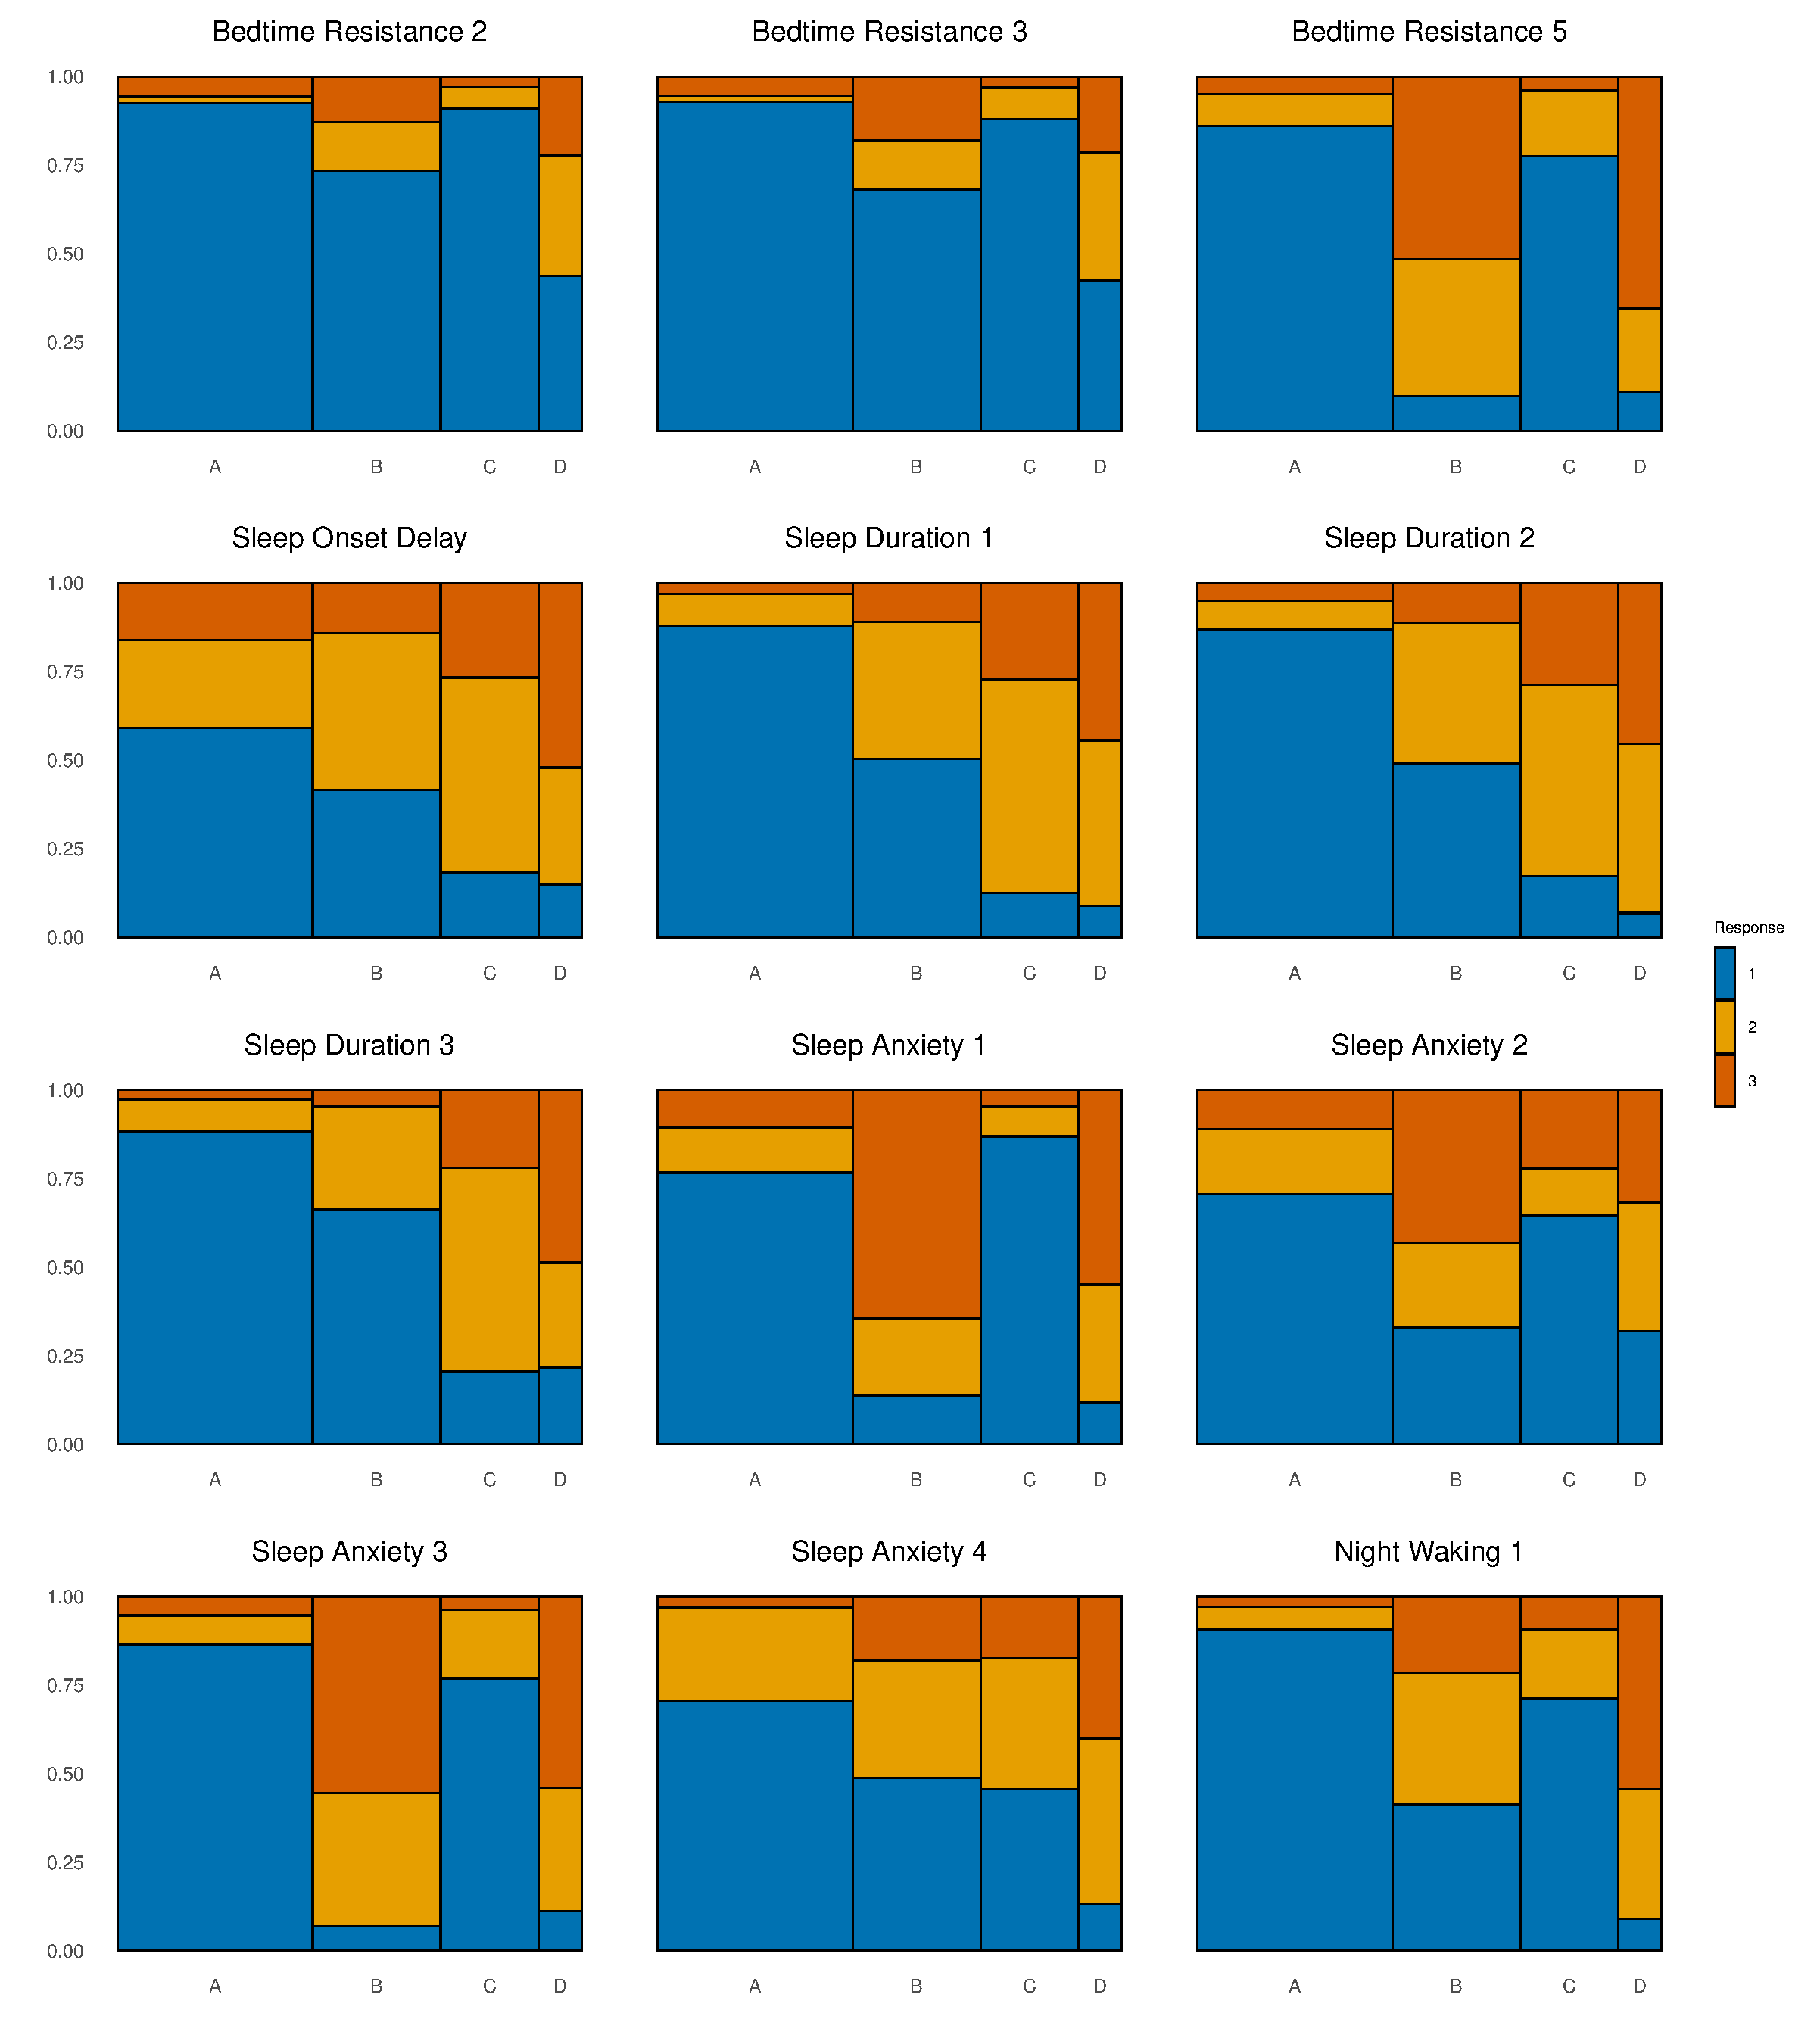
\includegraphics[width=\linewidth]{CSHQ_plots/CSHQ_mosaicplots_full/CSHQ_full_grid_LCA_mosaic1.pdf}
    \caption{}\label{fig:CSHQ_full_mosaic1}
\end{figure}

\begin{figure}[H]
    \centering
    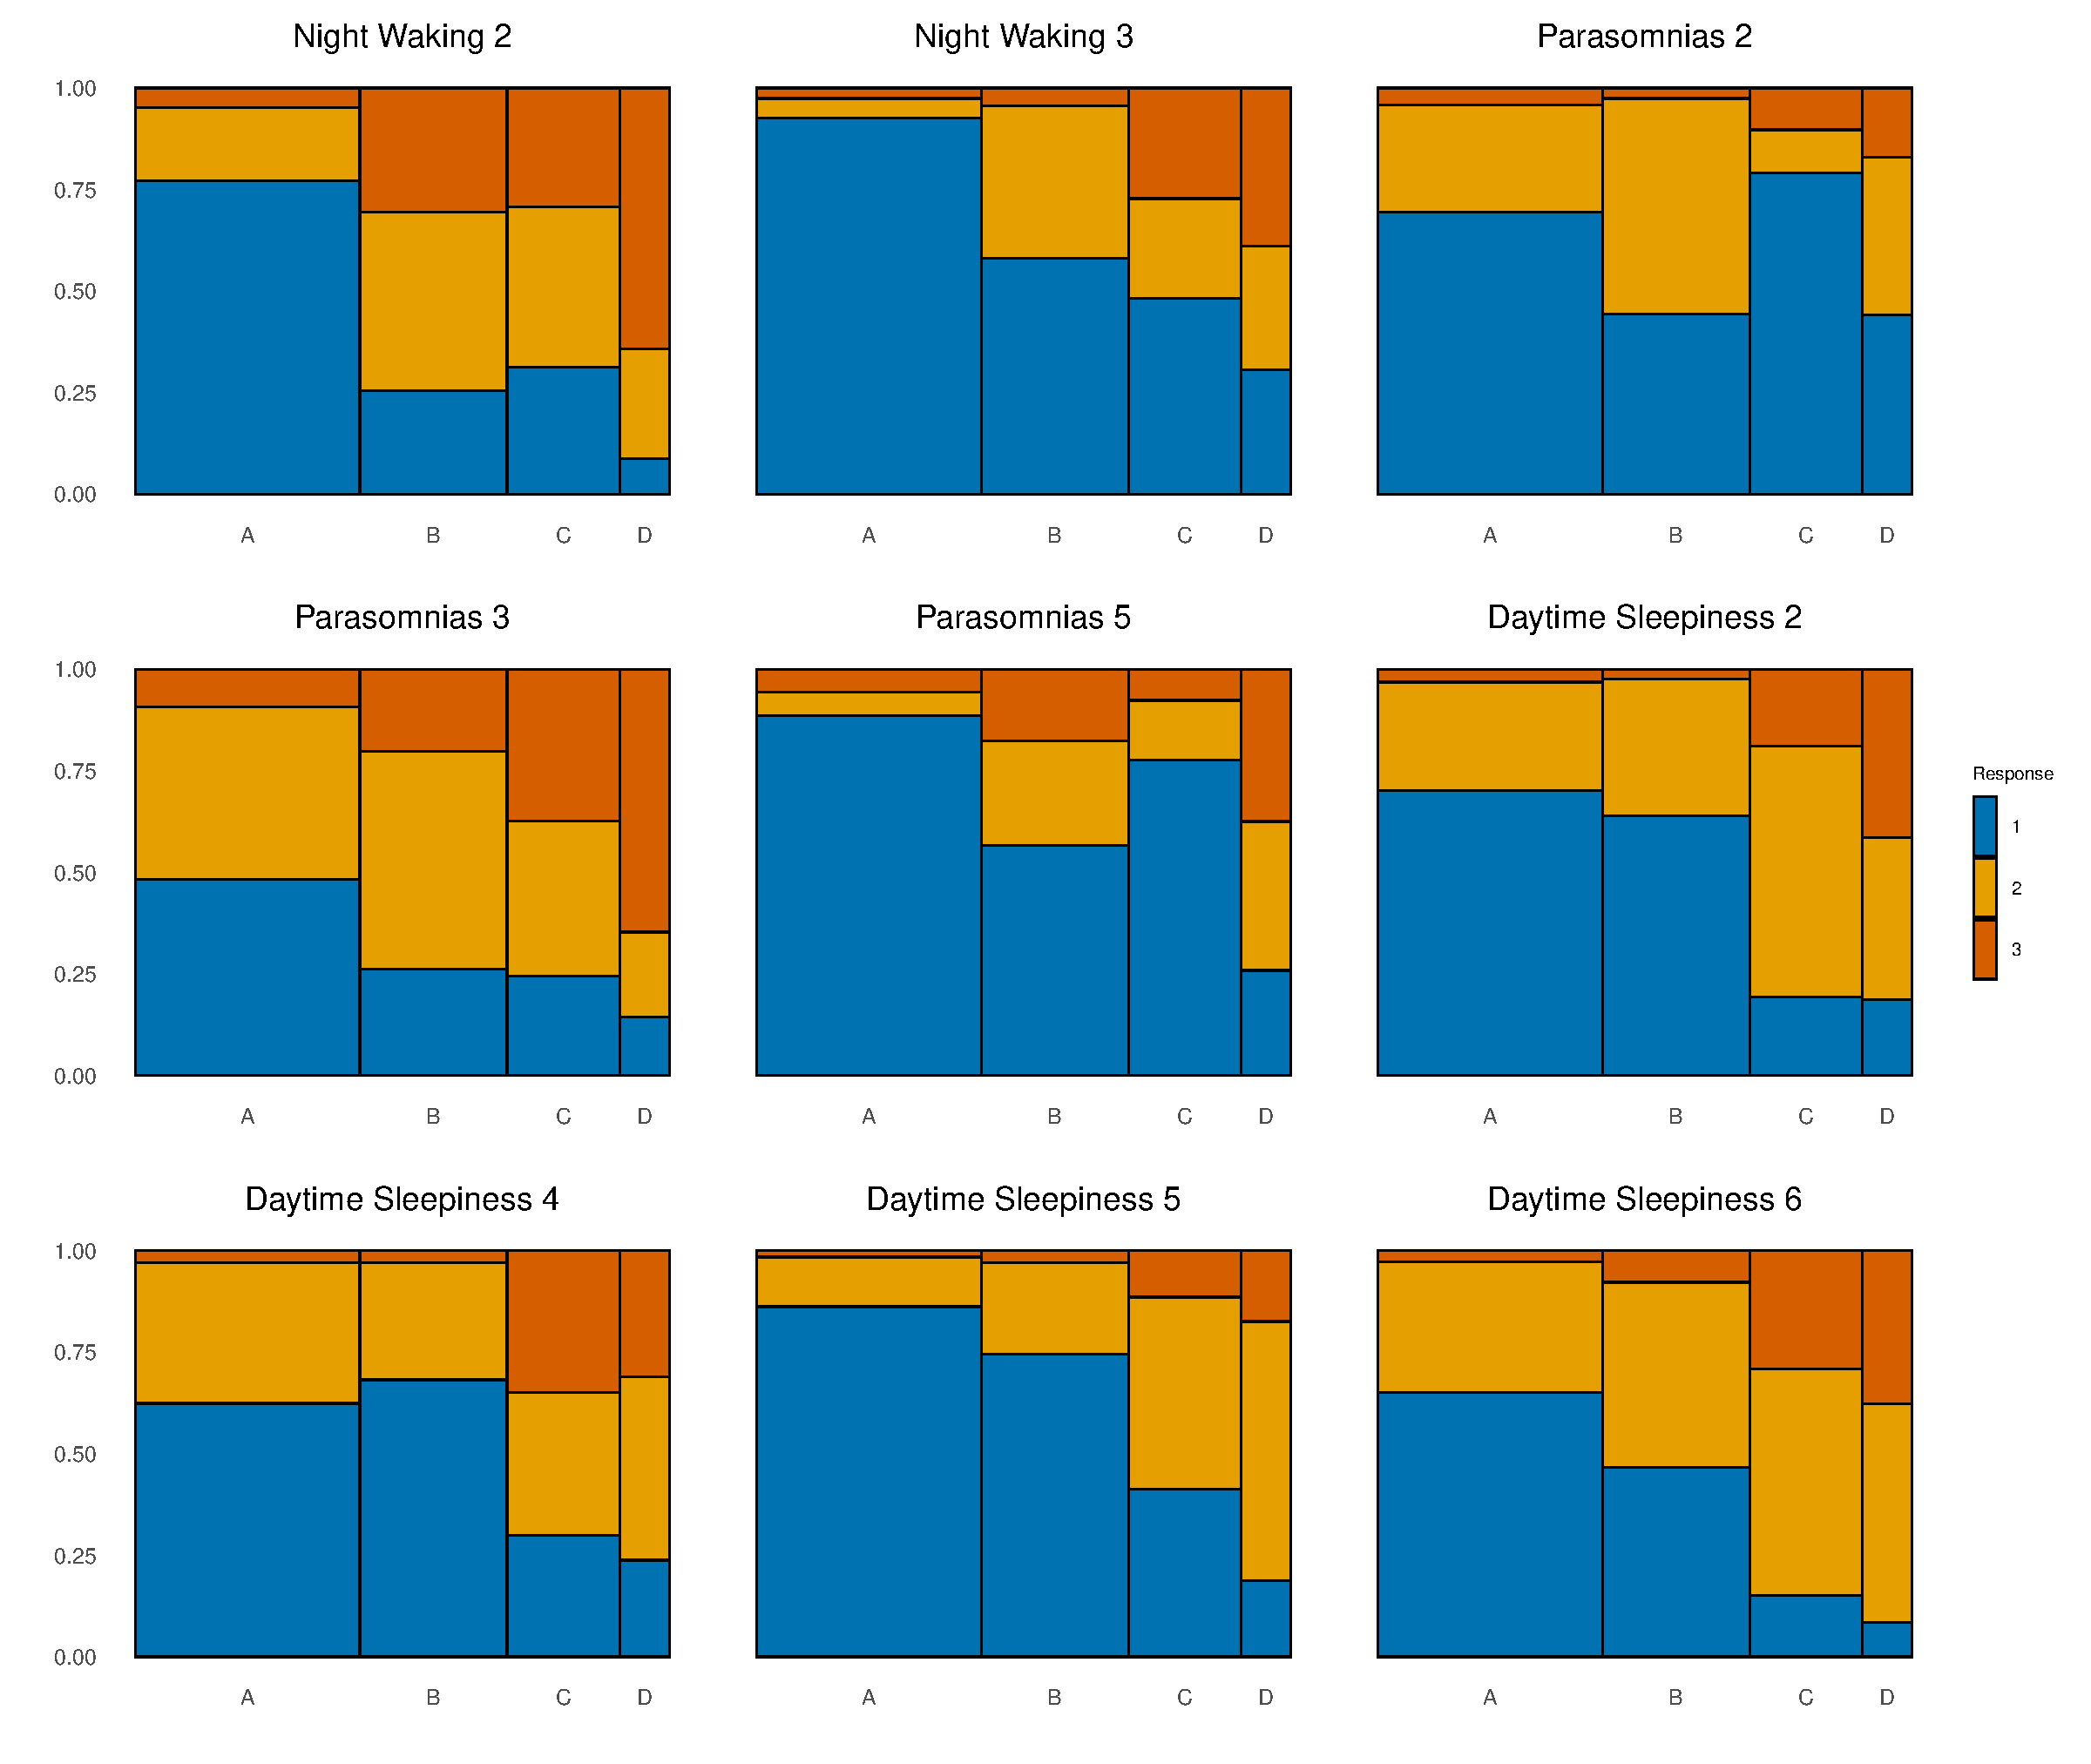
\includegraphics[width=\linewidth]{CSHQ_plots/CSHQ_mosaicplots_full/CSHQ_full_grid_LCA_mosaic2.pdf}
    \caption{}\label{fig:CSHQ_full_mosaic2}
\end{figure}



\section{Technical Derivations}

\subsection{Derivation of Pólya-Gamma Sampling Method for LCR}
This follows the method of \cite{polson_bayesian_2013}. Consider the full conditional for $\bsbet$ from (4). We can consider each of the $\bsbet_g$ parameters conditional on $\bsbet_{-g}$, the $\bsbet$ matrix with the $g$-th column removed. We write the expression for the full conditional distribution of $\bsbet_g$ as
\begin{equation}\label{beta_fc2}
p(\bsbet_g \mid \bsbet_{-g}, \boldX, \boldY) \propto p(\bsbet_g) \prod_{i=1}^n \left[  \frac{\exp(\boldX_i^T \bsbet_g)}{\sum_{h=1}^G \exp(\boldX_i^T \bsbet_h)}\right]^{z_{ig}}\left[1- \frac{\exp(\boldX_i^T \bsbet_g)}{\sum_{h=1}^G \exp(\boldX_i^T \bsbet_h)}\right]^{1-z_{ig}}.
\end{equation}
This can be rewritten in the form
\[
p(\bsbet_g \mid \bsbet_{-g}, \boldX, \boldZ) \propto p(\bsbet_g) \prod_{i=1}^n \frac{\exp(\eta_{ig})^{z_{ig}}}{1+\exp(\eta_{ig})},
\]
where
\[
\eta_{ig} = \boldX_i^T\bsbet_g - C_{ig}, \qquad C_{ig} = \log\left( \sum_{h \neq g} \exp(\boldX_i^T \bsbet_h) \right).
\]
By utilising the result from (5), we can introduce the Pólya-Gamma random variables $\omega_{ig} \sim \pg(1,0)$ for each $i = 1,\dots,n, g = 1,\dots,G-1$, which allows us to rewrite the full conditional as 
\[
p(\bsbet_g \mid \bsbet_{-g},\boldX, \boldY) 
\propto p(\bsbet_g) \prod_{i=1}^n \exp\left( \kappa_{ig}\eta_{ig} - \frac{\omega_{ig}\eta_{ig}^2}{2} \right),
\]
where $\kappa_{ig} = z_{ig} - \frac{1}{2}$. We can recognise the second multiplicative term here as a product of Gaussian kernels in the $\eta$ variables. By setting the prior $\bsbet_g \sim \cN(\mathbf{m}_{0g}, \mathbf{V}_{0g})$, we are left with a two part update for $\bsbet_g$ and $\omega_{ig}$, given by
 \begin{equation}
 \begin{aligned}
    \bsbet_g \mid \bsbet_{-g}, \omega_{\cdot g}, \boldX,\boldZ  &\sim \cN(\mathbf{m}_g, \mathbf{V}_g),\\
    \omega_{ig} \mid \bsbet, \boldX_i &\sim \pg(1,\eta_{ig}).
\end{aligned}
\end{equation}
where
\[
\mathbf{V}_g^{-1} = \boldX^T \Omega_g \boldX + \boldV_{0g}^{-1}, \qquad \boldm_g = \boldV_g \left( \boldX^T(\bskap_g+ \Omega_g\boldC_{\cdot g}) + \boldV_{0g}^{-1}\boldm_{0g} \right), \qquad \Omega_g = \diag(\{\omega_{ig}\}_{i=1}^n),
\]
and $\boldC_{\cdot g}$ is the $g$-th column of $\boldC = (C_{ig})$.

\bibliographystyle{apalike-doi} 
\bibliography{references}       
\end{document}
